% Colors
\definecolor{colGreen}{RGB}{34,153,84}
\definecolor{colYellow}{RGB}{245,189,72}
\definecolor{colPink}{RGB}{219,50,120}
\definecolor{colGray}{RGB}{190,190,190}
\definecolor{colBlack}{RGB}{30,30,30}

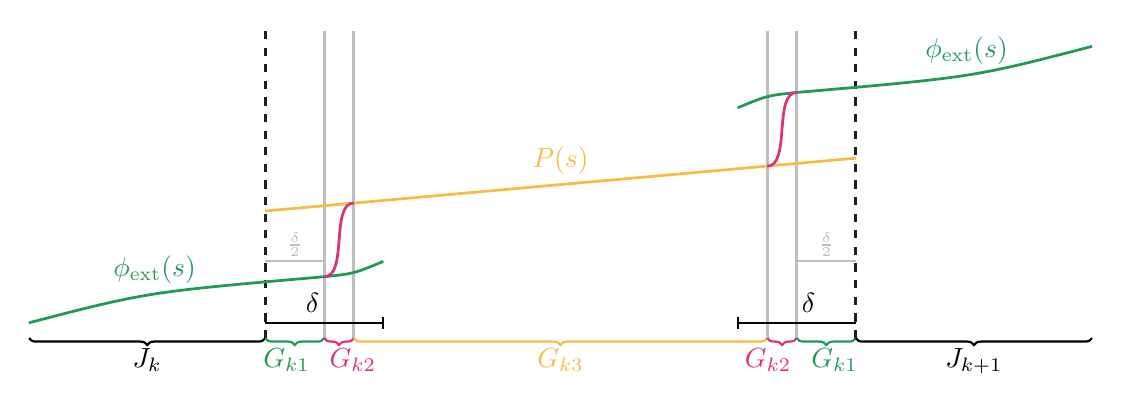
\begin{tikzpicture}[x=1.5cm, y=1.3cm]

% Parameters
\def\xL{0}      % Left vertical x posx
\def\xR{5}      % Right vertical x pos
\def\hV{3}      % Height of verticals
\def\yBase{0}   % Baseline y
\def\dlt{1}     % Delta length


% Vertical dashed lines
\foreach \x in {\xL, \xR} {
    \draw[line width=1pt, colBlack, dashed] (\x, \yBase) -- ++(0, \hV);
}

% Vertical delta lines
\foreach \dx in {0.5, 0.75} {
    \draw[line width=1pt, colGray] (\xL+\dx*\dlt, 0) -- ++(0, \hV);
    \draw[line width=1pt, colGray] (\xR-\dx*\dlt, 0) -- ++(0, \hV);
}

% Horizontal delta lines and labels
% Left delta
\draw[line width=0.7pt] (\xL, 0.05*\hV) -- ++(\dlt, 0)
    node [pos=0.4, anchor=south] {$\delta$};
\draw[line width=0.7pt] (\xL+\dlt, 0.03*\hV) -- ++(0, 0.04*\hV);

% Right delta
\draw[line width=0.7pt] (\xR, 0.05*\hV) -- ++(-\dlt, 0)
    node [pos=0.4, anchor=south] {$\delta$};
\draw[line width=0.7pt] (\xR-\dlt, 0.03*\hV) -- ++(0, 0.04*\hV);

% Delta/2 lines
\draw[colGray, line width=0.8pt] (\xL, 0.25*\hV) -- ++(0.5*\dlt, 0)
    node [pos=0.5, anchor=south, yshift=-2] {\scriptsize $\frac{\delta}{2}$};
\draw[colGray, line width=0.8pt] (\xR, 0.25*\hV) -- ++(-0.5*\dlt, 0)
    node [pos=0.5, anchor=south, yshift=-2] {\scriptsize $\frac{\delta}{2}$};


% P(s)
\draw[line width=1pt, colYellow] (\xL, 0.414*\hV) -- (\xR, 0.586*\hV)
    node [pos=0.5, anchor=south] {$P(s)$};


% phi_ext(s) curves
% Left
\draw[line width=1pt, colGreen] (\xL-2*\dlt, 0.05*\hV)
    .. controls (\xL-\dlt, 0.15*\hV) .. (\xL+0.5*\dlt, 0.2*\hV)
    node [pos=0.5, anchor=south] {$\phi_{\mathrm{ext}}(s)$}
    .. controls (\xL+0.75*\dlt, 0.21*\hV) .. (\xL+\dlt, 0.25*\hV);

% Right
\draw[line width=1pt, colGreen] (\xR+2*\dlt, 0.95*\hV)
    .. controls (\xR+\dlt, 0.85*\hV) .. (\xR-0.5*\dlt, 0.8*\hV)
    node [pos=0.5, anchor=south] {$\phi_{\mathrm{ext}}(s)$}
    .. controls (\xR-0.75*\dlt, 0.79*\hV) .. (\xR-\dlt, 0.75*\hV);

    
% Small S-shaped transitions (interpolations)
% Left
\draw[line width=1pt, colPink] (\xL+0.5*\dlt, 0.2*\hV)
    .. controls (\xL+0.7*\dlt, 0.2*\hV) and (\xL+0.55*\dlt, 0.44*\hV)
    .. (\xL+0.75*\dlt, 0.44*\hV);

% Right
\draw[line width=1pt, colPink] (\xR-0.5*\dlt, 0.8*\hV)
    .. controls (\xR-0.7*\dlt, 0.8*\hV) and (\xR-0.55*\dlt, 0.56*\hV)
    .. (\xR-0.75*\dlt, 0.56*\hV);


% Underbraces with labels
\draw[thick, decoration={brace, mirror}, decorate]
    (\xL-2*\dlt, 0) -- (\xL, 0)
    node [pos=0.5, anchor=north] {$J_{k}$};

\draw[colGreen, thick, decoration={brace, mirror}, decorate]
    (\xL, 0) -- (\xL+0.5*\dlt, 0)
    node [pos=0.5, anchor=north, xshift=-3] {$G_{k1}$};

\draw[colPink, thick, decoration={brace, mirror}, decorate]
    (\xL+0.5*\dlt, 0) -- (\xL+0.75*\dlt, 0)
    node [pos=0.5, anchor=north, xshift=5] {$G_{k2}$};

\draw[colYellow, thick, decoration={brace, mirror}, decorate]
    (\xL+0.75*\dlt, 0) -- (\xR-0.75*\dlt, 0)
    node [pos=0.5, anchor=north] {$G_{k3}$};

\draw[colPink, thick, decoration={brace}, decorate]
    (\xR-0.5*\dlt, 0) -- (\xR-0.75*\dlt, 0)
    node [pos=0.5, anchor=north, xshift=-5] {$G_{k2}$};

\draw[colGreen, thick, decoration={brace}, decorate]
    (\xR, 0) -- (\xR-0.5*\dlt, 0)
    node [pos=0.5, anchor=north, xshift=3] {$G_{k1}$};

\draw[thick, decoration={brace, mirror}, decorate]
    (\xR, 0) -- (\xR+2*\dlt, 0)
    node [pos=0.5, anchor=north] {$J_{k+1}$};

\end{tikzpicture}
